\documentclass{beamer}
\mode<presentation>
\usetheme{CambridgeUS}
\usepackage[russian]{babel}
\usepackage[utf8]{inputenc}
\usepackage[T2A]{fontenc}
\usepackage{sansmathaccent}

\usepackage{verbatim}
\usepackage{alltt}

\pdfmapfile{+sansmathaccent.map}
\title[Artifical Intelligence]{Поиск путей в искуственном интеллекте}
\author{Наумов Д.А., доц. каф. КТ}
\date[08.10.2019] {Экспертные системы и искусственный интеллект, 2019}

\begin{document}

%ТИТУЛЬНЫЙ СЛАЙД
\begin{frame}
  \titlepage
\end{frame}
  
%СОДЕРЖАНИЕ ЛЕКЦИИ
\begin{frame}
  \frametitle{Содержание лекции}
  \tableofcontents  
\end{frame}

\begin{frame}{Поиск пути}
Чтобы решить задачу, когда нет ясного вычисления допустимых решений, используетмся поиск пути.
\begin{itemize}
\item с помощью деревьев игр для игр с двумя игроками;
\item с помощью деревьев поиска для игр для одного игрока.
\end{itemize}
Эти подходы опираются на дерево состояния:
\begin{itemize}
\item корневой узел - начальное состояние
\item ребра - потенциальные ходы, которые преобразуют состояние в новое состояние. 
\end{itemize}
\end{frame}

\begin{frame}{Дерево игры}
Поиск  - сложная проблема, базовая структура не вычисляется полностью из-за взрывного роста количества состояний. Шашки $5\dot10^20$ различных позиций на доске. Деревья, в которых выполняется поиск, строятся по требованию по мере необходимости.
\begin{block}{Дерево игры}
\begin{itemize}
\item Два игрока по очереди выполняют ходы, которые изменяют состояние игры из ее первоначального состояния. 
\item Есть много состояний, в которых любой игрок может выиграть в игре. 
\item Могут быть некоторые состояния <<ничьей>>, в которых не выигрывает никто. 
\item Алгоритмы поиска пути увеличивают шанс, что игрок выиграет или обеспечит ничью.
\end{itemize}
\end{block}
\end{frame}

\begin{frame}
\begin{block}{Дерево поиска}
\begin{itemize}
\item Один игрок начинает игру с некоторого начального состояния и делает допустимые ходы до достижения желаемого целевого состояния. 
\item Алгоритм поиска пути определяет точную последовательность ходов, которые преобразуют исходное состояние в целевое.
\end{itemize}
\end{block}
Крестики-нолики: 765 уникальных позиций (без учета отражений и поворотов), 26830 возможнных игр.
\begin{figure}[h]
\centering
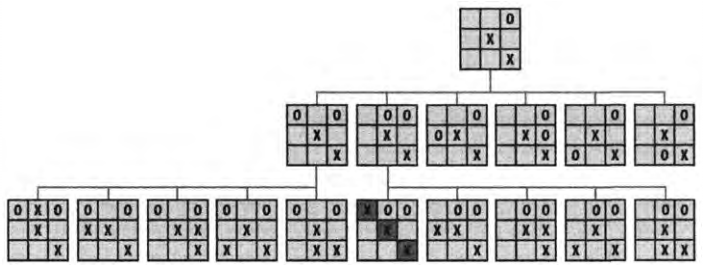
\includegraphics[scale=0.5]{images/lec05-pic01.png}
\end{figure}
\end{frame}

\begin{frame}
Дерево игры известно также как дерево И/ИЛИ, поскольку оно образуется из
двух различных типов узлов.
\begin{figure}[h]
\centering
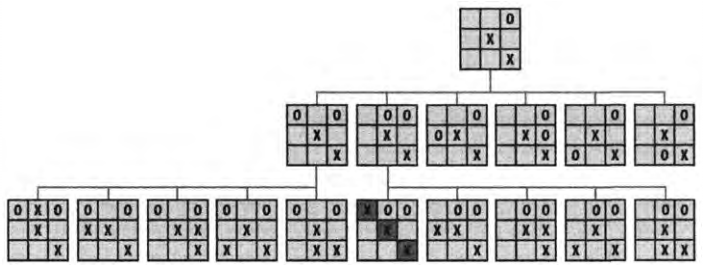
\includegraphics[scale=0.5]{images/lec05-pic01.png}
\end{figure}
\begin{itemize}
\item Верхний узел является узлом ИЛИ, так как целью игрока О является выбор только одного из шести доступных ходов на среднем уровне.
\item Узлы среднего уровня являются узлами И, потому что цель (с точки зрения игрока 0)
состоит в том, чтобы убедиться, что все ходы противника (показанные как дочерние
узлы на нижнем уровне) по-прежнему приведут к победе 0 или ничьей. 
\end{itemize}
\end{frame}

\begin{frame}
\begin{itemize}
\item В сложной игре дерево игры никогда не может быть вычислено полностью изза его размера. \item Целью алгоритма поиска пути является определение на основе состояния игры хода игрока, который максимизирует его шансы на победу в игре (или даже гарантирует ее). 
\item Таким образом, мы преобразуем множество решений игрока в задачу поиска пути в дереве игры.
\end{itemize}
Пример: игра в шашки
\begin{itemize}
\item доска размером 8x8 с начальным набором из 24 шашек (12 белых и 12 черных).
\item может ли игрок, делающий первый ход, обеспечить ничью или победу?
\item Schaeffer, J., N. Burch, Y. Bjornsson, A. Kishimoto, M. Muller, R. Lake, P Lu, and S. Sutphen, <<Checkers is solved>>, Science Magazine, September 14, 2007, 317(5844): 1518-1522,
http://www.sciencemag.org/cgi/content/abstract/317/5844/1518.
\end{itemize}
\end{frame}

\begin{frame}
Два типа подходов для поиска задач поиска: 
\begin{block}{Тип А}
\begin{itemize}
\item Рассмотрим различные разрешенные ходы для обоих игроков для фиксированного количества будущих ходов и определим наиболее благоприятное положение, получающееся в результате для исходного игрока. 
\item Затем выберем начальный ход, который движет игру в этом направлении.
\end{itemize}
\end{block}
Shannon, C., <<Programming a computer for playing chess>>, Philosophical Magazine,
41(314): 1950, http: //tinyurl.com/ChessShannon-pdf.
\end{frame}

\begin{frame}
\begin{block}{Тип Б}
\begin{itemize}
\item Добавим некоторые адаптивные решения, основанные на знании игры, а не
на статических оценках. 
\item Говоря более точно, а) оценим перспективные позиции на столько ходов вперед, сколько необходимо для выявления устойчивой позиции, в которой вычисления действительно отражают силу полученной позиции, и 6) выберем подходящие доступные ходы. 
\item Этот подход пытается предотвратить возможность бессмысленной траты драгоценного времени
\end{itemize}
\end{block}
Рассмотрим семейство алгоритмов типа А, который предоставляет
подход общего назначения для поиска в дереве игры наилучшего хода для игрока
в игре с двумя игроками. 
\begin{itemize}
\item Minimax;
\item AlphaBeta;
\item NegMax.
\end{itemize}
\end{frame}

\begin{frame}
Существует несколько способов сделать поиск более интеллектуальным:
\begin{itemize}
\item Выбор порядка и количества применяемых разрешенных ходов
	\begin{itemize}
	\item При рассмотрении доступных ходов для данного состояния игры сначала следует вычислить ходы, которые вероятнее других приведут к успешным результатам. 
	\item Кроме того, можно отказаться от определенных ходов, которые заведомо не приводят к успешным результатам.
	\end{itemize}
\item Выбор состояния игры для <<обрезки>> дерева поиска
	\begin{itemize}
	\item По мере выполнения поиска может быть обнаружена новая информация, которую можно использовать для устранения состояний игры, которые (в некоторый момент времени) были выбраны в качестве части поиска.
	\end{itemize}
\end{itemize}
\end{frame}

\begin{frame}
\begin{block}{Функция статических оценок}
оценивает состояния игры в промежуточных точках в процессе вычислений с последующим упорядочением множества доступных ходов так, чтобы сначала испытывались ходы, с более высокой вероятностью ведущие к выигрышу
\end{block}
Функция статической оценки должна:
\begin{itemize}
\item учитывать различные особенности позиции в дереве игры 
\item возвращать целочисленный балл, который отражает относительную силу позиции с точки зрения игрока. 
\end{itemize} 
Samuel, A., <<Some studies in machine learning using the game of checkers>>, IBM Journal
3(3): 210-229, 1967, http://dx.doi.org/10.1147/rd.116.0601.
\begin{itemize}
\item оценка позиции на доске путем рассмотрения двух десятков параметров, таких как сравнение количества шашек у игрока и его противника или возможностей размена шашек.
\end{itemize}
\end{frame}

\begin{frame}{Крестики-нолики}
Функция BoardEvaluation, определенная Нилом Нильссоном. Nilsson, N., Problem-Solving Methods in Artificial Intelligence. McGraw-Hill, 1971

Пусть nc(gs,p) — количество строк, столбцов или диагоналей в состоянии игры gs, в которых игрок р все еще может выстроить в ряд три своих значка. 

Затем мы определим score(gs, p) следующим образом:
\begin{itemize}
\item $+\infty$ - если игрок р победил в игре в состоянии gs;
\item $-\infty$ - если противник игрока р победил в игре в состоянии gs;
\item $nc{gs,p}-nc(gs, opponent)$ - если ни один игрок в состоянии игры gs не победил.
\end{itemize}
\end{frame}

\section{Концепция поиска путей}

\begin{frame}{Представление состояния}
Каждый узел дерева игры или дерева поиска содержит всю информацию о состоянии, известную как позиция в игре.

Пример: шахматы, рокировка возможно, если:
\begin{enumerate}
\item ни одна из этих фигур еще не делала хода, 
\item промежуточные клетки доски пустые и в настоящее время не находятся под боем фигур противника 
\item король в настоящее время не находится под шахом. 
\end{enumerate}

Состояние игры:
\begin{itemize}
\item должно храниться наиболее компактно;
\item может быть значительно уменьшено путем удаления эквивалентных состояний, которые можно получить простым поворотом или отражением
\end{itemize}
Cложные представления для шахмат или шашек: 
Pepicelli, G., <<Bitwise optimization in Java: Bitfields, bitboards, and beyond,>> O’Reilly on Java.com, February 2, 2005, http://www.onjava.com/pub/a/onjava/2005/02/02/bitsets.html.
\end{frame}

\begin{frame}{Вычисление доступных ходов}
Чтобы найти наилучший ход, в каждом состоянии должно быть возможно вычисление доступных ходов игрока.
\begin{block}{Коэффициент ветвления}
среднее количество ходов, которые разрешены из отдельного состояния.
\end{block}
\begin{itemize}
\item кубик Рубика - 13,50
\item четыре в ряд - 7,00
\item шашки - 6,14 (1,20 для позиций со взятием, 7,94 без взятия)
\item Го - 361,00
\end{itemize}
Если коэффициент ветвления у игры оказывается высоким, а ходы не упорядочены должным образом на основе некоторой вычисляемой меры успеха, слепой поиск
в дерева оказывается неэффективным.
\end{frame}

\begin{frame}{Максимальная глубина расширения}
\begin{itemize}
\item Из-за ограниченных ресурсов памяти некоторые алгоритмы поиска ограничивает
степень расширения деревьев поиска и игр.
\item Этот подход проявляет свою слабость, в первую очередь, в играх, в которых продуманная стратегия формируется с помощью последовательности ходов.
\item Фиксированная глубина расширения формирует <<горизонт>>, за который поиск не может заглянуть, и это часто препятствует успешному поиску. 
\item Для игр с одним игроком фиксация максимальной глубины означает, что алгоритм не в состоянии найти решение, которое лежит сразу за горизонтом.
\end{itemize}
Например, в шахматах нередка жертва фигуры
для получения потенциальных преимуществ. Если эта жертва происходит на краю
максимального расширения, выгодное состояние игры может не быть обнаружено.
\end{frame}

\section{Minimax}

\begin{frame}{Minimax}
\begin{itemize}
\item Для заданной конкретной позиции в дереве игры с точки зрения начального
игрока программа поиска должна найти ход, который привел бы к наибольшим шансам на победу (или хотя бы на ничью). 
\item Но вместо только текущего состояния игры
и доступных для этого состояния ходов программа должна рассматривать любые
ходы противника, которые он делает после хода нашего игрока. 
\end{itemize}
\begin{figure}[h]
\centering
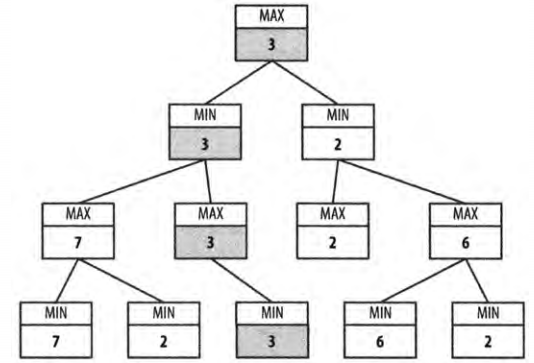
\includegraphics[scale=0.4]{images/lec05-pic02.png}
\end{figure}
\end{frame}

\begin{frame}{Minimax}
\begin{itemize}
\item функция оценки score (state, player), которая возвращает
целое число, представляющее оценку состояния игры с точки зрения игрока player;
\item дерево игры расширяется путем рассмотрения будущих состояний игры после
последовательности из n ходов. 
\item Каждый уровень дерева по очереди представляет собой уровень МАХ (на котором цель заключается в обеспечении выгоды для исходного игрока путем максимизации вычисленного состояния игры) и MIN (на котором цель заключается в обеспечении выгоды для противника путем минимизации вычисленного состояния игры). 
\item На чередующихся уровнях программа выбирает ход, который максимизирует score (state, initial), но на следующем уровне она
предполагает, что противник будет выбирать ход, который минимизирует значение
score(state, initial).
\end{itemize}
\end{frame}

\begin{frame}{Minimax}
\begin{itemize}
\item функция оценки score (state, player), которая возвращает
целое число, представляющее оценку состояния игры с точки зрения игрока player;
\item дерево игры расширяется путем рассмотрения будущих состояний игры после
последовательности из n ходов. 
\item Каждый уровень дерева по очереди представляет собой уровень МАХ (на котором цель заключается в обеспечении выгоды для исходного игрока путем максимизации вычисленного состояния игры) и MIN (на котором цель заключается в обеспечении выгоды для противника путем минимизации вычисленного состояния игры). 
\item На чередующихся уровнях программа выбирает ход, который максимизирует score (state, initial), но на следующем уровне она
предполагает, что противник будет выбирать ход, который минимизирует значение
score(state, initial).
\end{itemize}
\end{frame}

\begin{frame}
\begin{figure}[h]
\centering
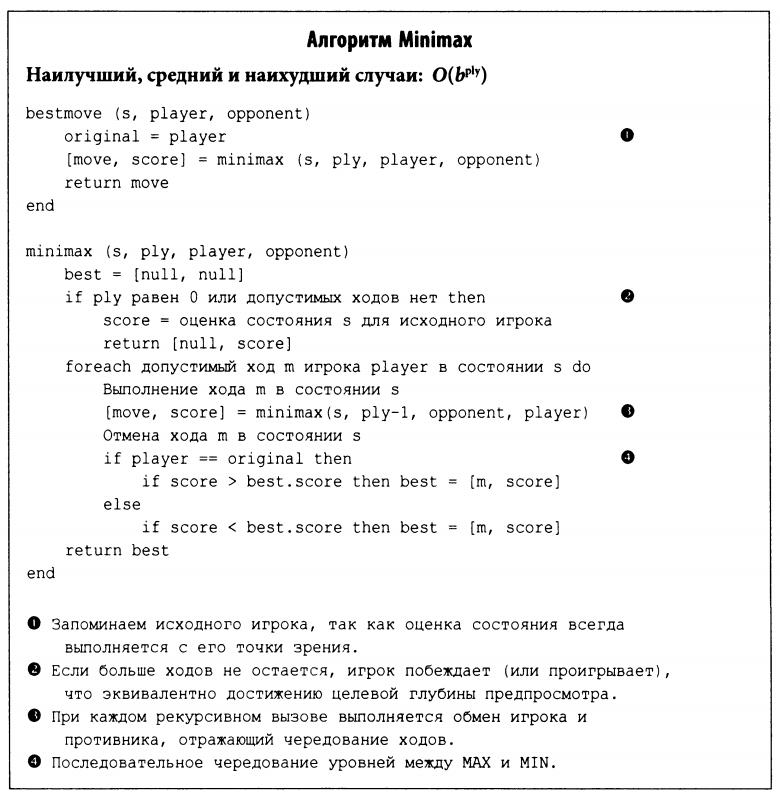
\includegraphics[scale=0.4]{images/lec05-pic03.png}
\end{figure}
\end{frame}

\begin{frame}
\begin{figure}[h]
\centering
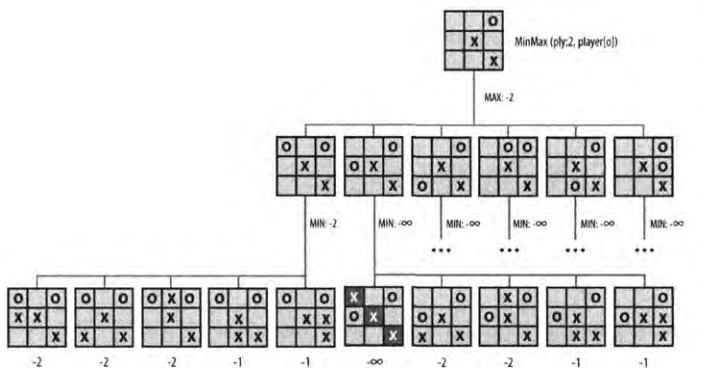
\includegraphics[scale=0.6]{images/lec05-pic04.png}
\end{figure}
\end{frame}

\begin{frame}{Анализ алгоритма Minimax}
\begin{itemize}
\item Если для каждого состояния игры имеется фиксированное количество ходов b
(или даже когда количество доступных ходов уменьшается на единицу с каждым
уровнем), общее количество состояний игры, в которых выполняется поиск при
предпросмотре глубиной d, представляет собой $O(b^n)$ демонстрируя экспоненциальный рост. 
\item Ограничения глубины предпросмотра могут быть устранены, если дерево
игры достаточно мало для полной оценки за приемлемый промежуток времени.
\item Поскольку мы предполагаем, что и игрок, и противник играют
без ошибок, мы должны найти способ остановить расширение дерева игры после
того, как алгоритм определяет, что дальнейшее изучение данного поддерева бессмысленно.
\end{itemize}
\end{frame}

\begin{frame}{NegMax}
\begin{itemize}
\item Алгоритм NegMax заменяет чередование уровней МАХ и MIN алгоритма Minimax
единым подходом, используемым на каждом уровне дерева игры.
\item Cостояние игры всегда оценивается с точки зрения игрока, делающего начальный ход (что требует от функции оценки хранения этой информации).
\item Алгоритм NegMax последовательно ищет ход, который дает
максимум из значений дочерних узлов состояния с обратным знаком.
\end{itemize}
\begin{figure}[h]
\centering
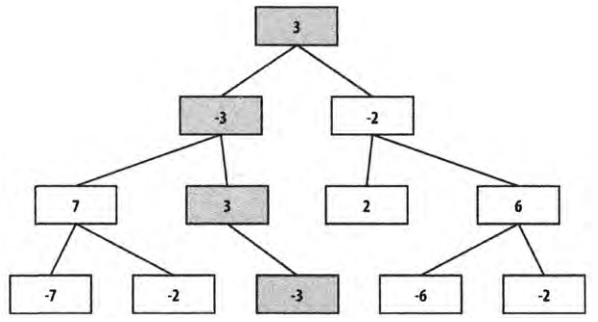
\includegraphics[scale=0.35]{images/lec05-pic05.png}
\end{figure}
\end{frame}

\begin{frame}{NegMax}
\begin{figure}[h]
\centering
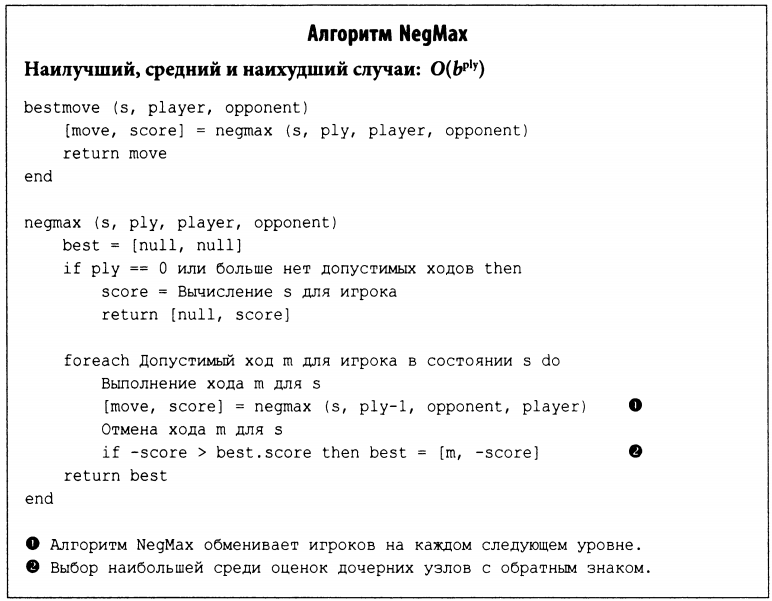
\includegraphics[scale=0.4]{images/lec05-pic06.png}
\end{figure}
\end{frame}

\begin{frame}{NegMax}
\begin{figure}[h]
\centering
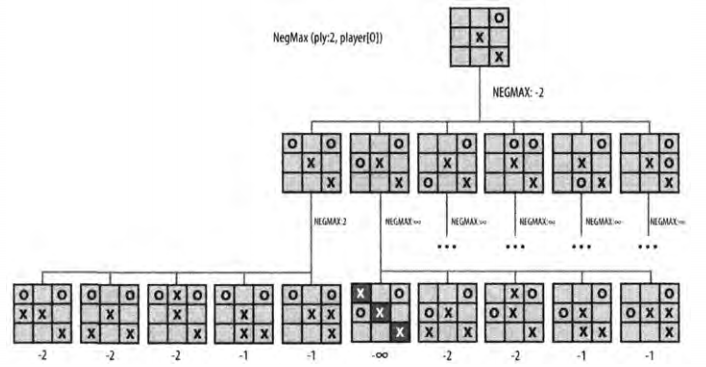
\includegraphics[scale=0.6]{images/lec05-pic07.png}
\end{figure}
\end{frame}

\begin{frame}{AlhaBeta}
Алгоритм AlphaBeta определяет стратегию последовательного обрезания всех непродуктивных поисков в дереве
\begin{figure}[h]
\centering
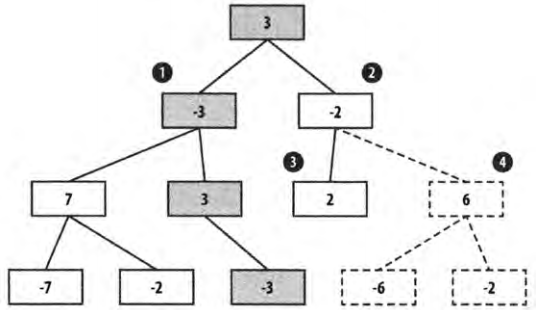
\includegraphics[scale=0.6]{images/lec05-pic08.png}
\end{figure}
\end{frame}

\begin{frame}{AlhaBeta}
\begin{itemize}
\item После оценки поддерева игры с корнем в (1) алгоритм AlphaBeta знает,
что если этот ход сделан, то противник не может сделать позицию хуже, чем -3.
\item Это означает, что лучшее, что может сделать игрок, — добиться состояния с оценкой 3. 
\item Когда AlphaBeta переходит в состояние игры (2), то его первый дочерний узел — состояние (3) — имеет оценку, равную 2. 
\item Это означает, что если выбрать ход, приводящий в (2), то противник может заставить игрока перейти в состояние игры с оценкой, меньшей, чем лучшая найденная к этому моменту (т.е. 3). 
\item Таким образом, не имеет смысла проверять поддерево с корнем в (4), и оно полностью отбрасывается.
\end{itemize}
\end{frame}

\begin{frame}{Предпросмотр AlhaBeta глубиной 2}
\begin{figure}[h]
\centering
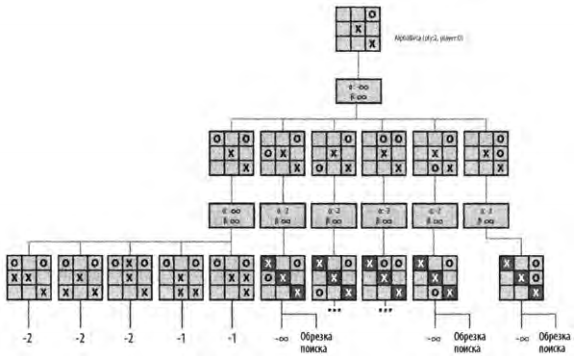
\includegraphics[scale=0.6]{images/lec05-pic09.png}
\end{figure}
\end{frame}

\begin{frame}{Предпросмотр AlhaBeta глубиной 2}
\begin{itemize}
\item Когда алгоритм AlphaBeta ищет лучший ход, он помнит, что X может
достичь оценки не выше 2, если О делает ход в левый верхний угол. 
\item Для каждого другого хода 0 AlphaBeta определяет, что X имеет хотя бы один ход, который превосходит первый ход 0 (на самом деле для всех прочих ходов 0 игрок X может победить).
\item Таким образом, дерево игры расширяется только до 16 узлов, что представляет собой экономию более 50\% по сравнению с алгоритмом Minimax. 
\end{itemize}
\end{frame}

\begin{frame}{Алгоритм AlhaBeta}
\begin{figure}[h]
\centering
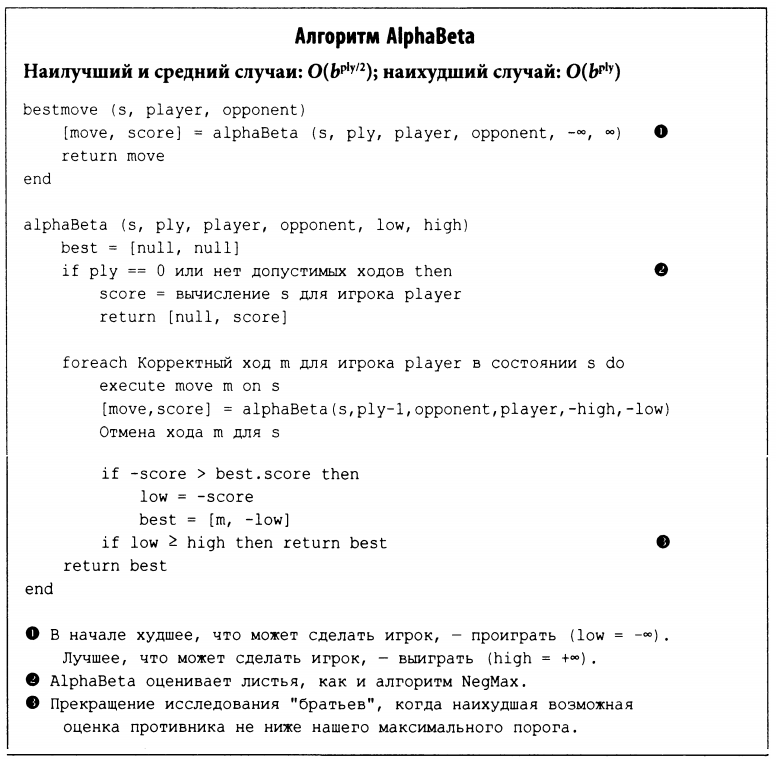
\includegraphics[scale=0.4]{images/lec05-pic10.png}
\end{figure}
\end{frame}

\begin{frame}{Алгоритм AlhaBeta}
\begin{itemize}
\item Алгоритм рекурсивно выполняет поиск в дереве игры и поддерживает
два значения, $\alpha$ и $\beta$, которые определяют <<окно возможностей>> для игрока до тех пор, пока $\alpha < beta$. 
\item Значение $\alpha$ представляет нижнюю границу состояний игры, найденную для игрока до настоящего времени (или $-\infty$, если ничего не было найдено)
и объявляет, что игрок нашел ход, гарантирующий, что он может достичь как минимум указанного значения. Более высокие значения $\alpha$ означают, что игрок поступает правильно; при $\alpha = +\infty$ игрок выиграл, и поиск можно завершать.
\item Значение $\beta$ представляет верхнюю границу состояний игры, найденную для игрока до настоящего времени (или $+\infty$, если ничего не было найдено) и объявляет максимальное значение, которого игрок может достичь. Если значение $\beta$ уменьшается все сильнее и сильнее, значит, противник поступает верно и делает наилучшие ходы, ограничивающие доступные для игрока варианты. 
\end{itemize}
\end{frame}

\begin{frame}{Алгоритм AlhaBeta}
\begin{figure}[h]
\centering
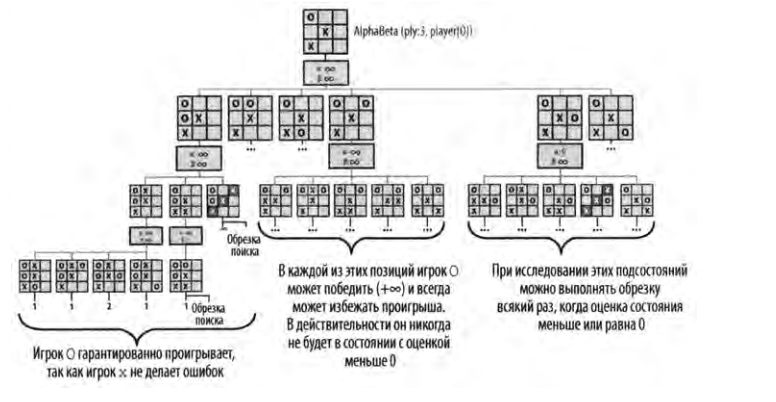
\includegraphics[scale=0.6]{images/lec05-pic11.png}
\end{figure}
\end{frame}

\begin{frame}{Анализ алгоритмов}
Пусть каждый раз игроки могут сделать b ходов, а алгоритм просматривает на d ходов вперед. 
\begin{itemize}
\item число вершин MinMax, NegMax - $b^d$;
\item AlphaBeta оценивает b состояний игры для начинающего игрока на каждом уровне, но только одно состояние игры — для его противника. 
\item число вершин для AlphaBeta - $b^(d/2)$.
\end{itemize}
Алгоритм AlphaBeta может также исследовать то же общее количество состояний игры, что и алгоритм Minimax, расширяя глубину дерева игры до 2d.
\begin{figure}[h]
\centering
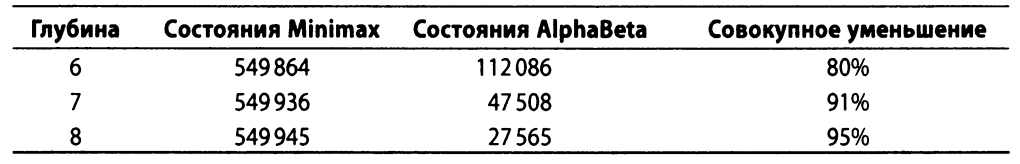
\includegraphics[scale=0.4]{images/lec05-pic12.png}
\end{figure}
Глубина предпросмотра $9—k$, которая гарантирует, что просмотрены все возможные ходы.
\end{frame}
\end{document}